\documentclass{article}
\usepackage{float}
\usepackage{hyperref}
\usepackage{geometry}
\usepackage{amsmath}
\usepackage{graphicx}
\geometry{a4paper, margin=1in}

\title{Software Requirements Specification (SRS) \\ ArmSpace Project}
\author{Your Name}
\date{June 14, 2025}

\begin{document}

\maketitle

\tableofcontents

\section{Introduction}
\subsection{Purpose}
This document defines the software requirements specification (SRS) for the \textbf{ArmSpace} project. It outlines the functionality, interfaces, constraints, and testing strategies required for the initial version of the system.

\subsection{Scope}
ArmSpace is a software tool designed to process structured input data, perform calculations via a computation engine, and provide motor control commands in JSON format.

\subsection{Definitions and Abbreviations}
\begin{itemize}
    \item \textbf{SRS}: Software Requirements Specification
    \item \textbf{JSON}: JavaScript Object Notation
    \item \textbf{CMake}: Cross-platform build system
    \item \textbf{gtest}: Google Test framework
    \item \textbf{Quaternion}: A mathematical representation for rotation, avoiding gimbal lock.
\end{itemize}

\section{Overall Description}
\subsection{System Architecture Overview}
The system consists of multiple **modules** working together:

\begin{itemize}
    \item \textbf{Input Parser}: Validates and processes JSON input files.
    \item \textbf{Computation Engine}: Handles quaternion-based calculations and motor tick conversion.
    \item \textbf{Logging System}: Uses \textbf{spdlog} for structured error reporting.
    \item \textbf{Output Generator}: Produces JSON-formatted motor control values.
\end{itemize}

\subsection{Architecture Diagram}
\begin{figure}[h]
    \centering
    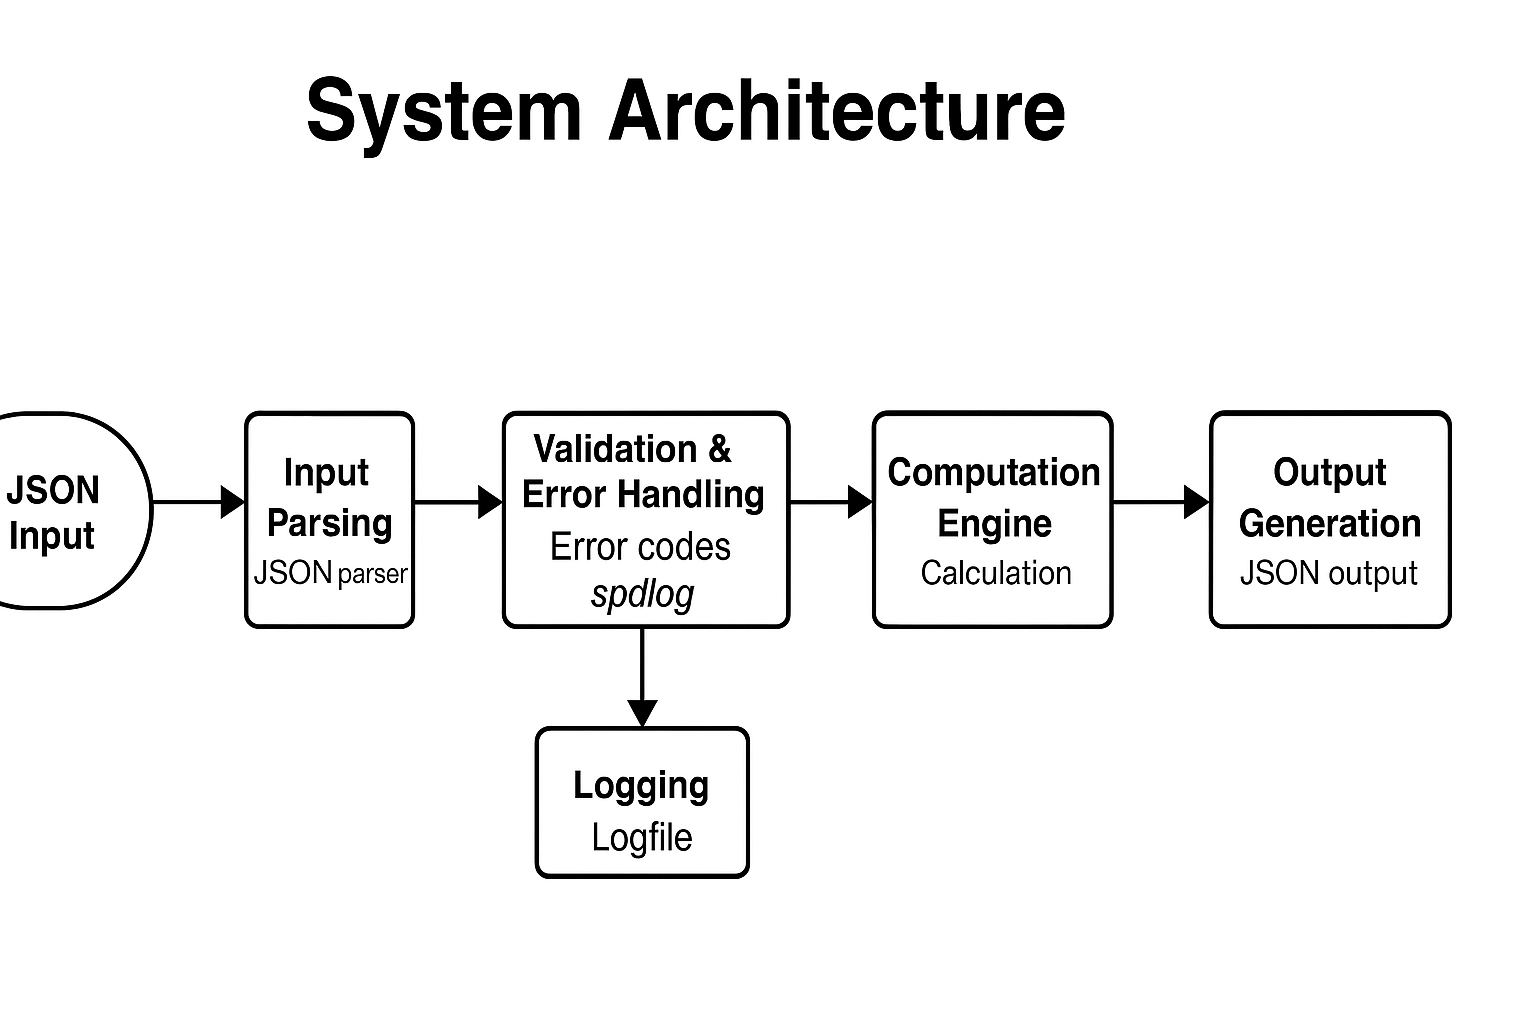
\includegraphics[width=0.8\textwidth]{architecture_diagram.png}
    \caption{ArmSpace System Architecture}
\end{figure}

\subsection{Supported Platforms}
ArmSpace is designed to run on:
\begin{itemize}
    \item **Linux**
    \item **macOS**
    \item **Windows**
\end{itemize}
Future versions may be ported to additional platforms.

\subsection{Constraints}
\begin{itemize}
    \item Implemented in C++
    \item Uses \textbf{nlohmann/json} for JSON parsing and writing
    \item Uses \textbf{spdlog} for logging
    \item Uses \textbf{CMake} as the build system for cross-compiling to Windows
    \item Input and output in JSON format
    \item Command-line interface (CLI) for the current version
\end{itemize}

\section{Project Folder Structure}
The following **organized directory layout** ensures clarity and maintainability:

\begin{itemize}
    \item \texttt{/src} – Source code files
    \item \texttt{/include} – Header files
    \item \texttt{/tests} – Unit and integration tests
    \item \texttt{/docs} – Documentation (SRS, readme, architecture diagram)
    \item \texttt{/logs} – Log files (saved runtime information)
    \item \texttt{/build} – Compiled binaries and intermediate files
    \item \texttt{/config} – JSON input/output examples
    \item \texttt{/schemas} – JSON schema files for validation
    \item \texttt{CMakeLists.txt} – CMake build configuration
    \item \texttt{README.md} – Project overview and instructions
\end{itemize}

\section{JSON Format Specification}
\subsection{Reading JSON from Command-Line Argument}
The system allows users to specify an **input JSON file** as a command-line argument, ensuring flexibility and avoiding hardcoded file paths.

\subsection{JSON Input Format}
The system expects a structured JSON input, describing joints, motors, and arm segments.

\begin{verbatim}
{
    "robot_name": "ArmSpaceBot",
    "joints": [
        {
            "name": "shoulder",
            "position": [0, 0, 0],
            "motors": [
                {
                    "name": "shoulder_motor_x",
                    "rotation_axis": [1, 0, 0],
                    "ticks_per_revolution": 1000
                },
                {
                    "name": "shoulder_motor_z",
                    "rotation_axis": [0, 0, 1],
                    "ticks_per_revolution": 1200
                }
            ],
            "arm_segment": { "length": 10, "direction": [1, 0, 0] }
        },
        {
            "name": "elbow",
            "position": [10, 0, 0],
            "motors": [
                {
                    "name": "elbow_motor_y",
                    "rotation_axis": [0, 1, 0],
                    "ticks_per_revolution": 1100
                },
                {
                    "name": "elbow_motor_x",
                    "rotation_axis": [1, 0, 0],
                    "ticks_per_revolution": 900
                }
            ],
            "arm_segment": { "length": 10, "direction": [1, 0, 0] }
        }
    ],
    "desired_position": [10, 7, 5]
}
\end{verbatim}

\subsection{JSON Output Format}
The system calculates movements based on quaternion-based rotations and outputs motor tick values.

\begin{verbatim}
{
    "motor_ticks": [
        { "name": "shoulder_motor_x", "ticks": 97 },
        { "name": "shoulder_motor_z", "ticks": 82 },
        { "name": "elbow_motor_y", "ticks": 100 },
        { "name": "elbow_motor_x", "ticks": 105 }
    ],
    "status": "adjusted",
    "final_position": [10, 6.9, 4.9]
}
\end{verbatim}

\section{Error Handling}
\subsection{Error Reporting and Logging}
Standardized error codes ensure structured fault recovery.

\begin{table}[H]
\centering
\begin{tabular}{|c|l|p{8cm}|}
\hline
\textbf{Error Code} & \textbf{Message} & \textbf{Description} \\
\hline
ERR001 & Invalid Arm Length & A joint position does not match the expected length \& direction. \\
\hline
ERR002 & Disconnected Joint & A joint is not properly connected to the sequence. \\
\hline
ERR003 & Malformed JSON & The input structure is incorrect or missing required fields. JSON parsing failed. \\
\hline
ERR004 & Motor Data Missing & A motor definition is missing configurations, preventing tick calculation. \\
\hline
ERR005 & Unsupported Joint Count & The number of joints exceeds the maximum limit (future constraint: 6). \\
\hline
ERR006 & Invalid Rotation Axis & A motor has an incorrectly formatted rotation axis (should be a unit vector). \\
\hline
ERR007 & Quaternion Calculation Failure & Rotation computations failed due to incorrect vector inputs. \\
\hline
ERR008 & Tick Calculation Overflow & The computed tick value exceeds the allowed motor range. \\
\hline
\end{tabular}
\caption{Complete error code table for validation and computation}
\end{table}

\subsection{JSON Error Response Format}
If an error occurs, the system returns a structured JSON error message.

\begin{verbatim}
{
    "error": "Invalid arm length",
    "details": "Joint 'elbow' is not reachable from 'shoulder' based on defined segment length."
}
\end{verbatim}

\section{Mathematical Formulation}
\subsection{Quaternion-Based Rotation Computation}
To ensure precise, stable transformations and prevent **gimbal lock**, the system computes joint rotations using quaternions.

\subsection{Quaternion Representation}
A quaternion is defined as:



\[
q = w + x\mathbf{i} + y\mathbf{j} + z\mathbf{k}
\]



where:
\begin{itemize}
    \item \( w \) is the scalar (real) component.
    \item \( x, y, z \) are the vector (imaginary) components along **X, Y, Z axes**.
\end{itemize}

\subsection{Computing Rotation Using Quaternions}
Given a rotation by angle \( \theta \) around a normalized axis \( \mathbf{a} = (a_x, a_y, a_z) \), the quaternion is:



\[
q = \cos(\theta/2) + (a_x\mathbf{i} + a_y\mathbf{j} + a_z\mathbf{k}) \sin(\theta/2)
\]



For a given vector \( P = (p_x, p_y, p_z) \), the rotated vector \( P' \) is computed using:



\[
P' = q P q^{-1}
\]



where \( q^{-1} \) is the inverse quaternion:



\[
q^{-1} = \frac{w - x\mathbf{i} - y\mathbf{j} - z\mathbf{k}}{||q||^2}
\]



\section{Example Calculation: Quaternion-Based Arm Rotation}
\subsection{Robot Configuration}
\begin{itemize}
    \item \textbf{Joint 1 (Shoulder)}: Positioned at \( (0, 0, 0) \), rotates **around Z-axis**.
    \item \textbf{Joint 2 (Elbow)}: Positioned at \( (10, 0, 0) \), rotates **around Y-axis**.
    \item \textbf{Arm segments}:
        \begin{itemize}
            \item Segment **1**: Length = 10, direction = \([1, 0, 0]\).
            \item Segment **2**: Length = 10, direction = \([1, 0, 0]\).
        \end{itemize}
    \item \textbf{Desired end-effector position}: \( (10, 7, 5) \).
\end{itemize}

\subsection{Computing Rotation Using Quaternions}
\textbf{Step 1: Convert Position Vectors to Quaternions}

\begin{itemize}
    \item Current vector: \( v_1 = [10, 0, 0] \).
    \item Target vector: \( v_2 = [10, 7, 5] \).
\end{itemize}

\textbf{Step 2: Compute Rotation Axis}

Using the **cross product**:



\[
\mathbf{axis} = v_1 \times v_2 = [0, -50, 70]
\]



Normalized:



\[
\mathbf{axis} = [0, -0.58, 0.82]
\]



\textbf{Step 3: Compute Rotation Angle}

Using the **dot product**:



\[
\theta = \cos^{-1} \left( \frac{10 \times 10 + 0 \times 7 + 0 \times 5}{|v_1| |v_2|} \right) = \cos^{-1} (0.81) \approx 35^\circ
\]



\textbf{Step 4: Compute Rotation Quaternion}



\[
q = \cos(\theta/2) + \sin(\theta/2) \cdot (0, -0.58, 0.82)
\]





\[
q = [0.98, 0, -0.29, 0.41]
\]



\textbf{Step 5: Apply Quaternion Transformation}



\[
P' = q P q^{-1}
\]



After calculations, the new joint position is **adjusted to** \( P' = [10, 6.9, 4.9] \), moving the arm toward the target **without gimbal lock**.

\subsection{Motor Tick Conversion}
Using motor resolution:



\[
\mathrm{Ticks} = \left(\frac{\theta \times \text{ticks\_per\_revolution}}{360} \right)
\]



For **shoulder** (motor resolution: **1000** ticks/rev):



\[
\mathrm{Ticks}_{\text{shoulder}} = \left(\frac{35 \times 1000}{360} \right) = 97
\]



For **elbow** (motor resolution: **1200** ticks/rev):



\[
\mathrm{Ticks}_{\text{elbow}} = \left(\frac{30 \times 1200}{360} \right) = 100
\]



\subsection{Final JSON Output}
\begin{verbatim}
{
    "motor_ticks": [
        { "name": "shoulder_motor_x", "ticks": 97 },
        { "name": "shoulder_motor_z", "ticks": 82 },
        { "name": "elbow_motor_y", "ticks": 100 },
        { "name": "elbow_motor_x", "ticks": 105 }
    ],
    "status": "adjusted",
    "final_position": [10, 6.9, 4.9]
}
\end{verbatim}



\section{Functional Requirements}
\begin{itemize}
  \item FR1: The system shall parse structured JSON input files.
  \item FR2: The system shall perform computations using the parsed input.
  \item FR3: The system shall generate structured output in JSON format.
  \item FR4: The system shall validate input and report errors clearly.
\end{itemize}

\section{Non-Functional Requirements}
\begin{itemize}
  \item NFR1: The system shall run on macOS and Windows platforms.
  \item NFR2: The system shall be written in portable C++.
  \item NFR3: The system shall process typical input within 2 seconds.
  \item NFR4: The system shall achieve a minimum of 90\% unit test coverage.
\end{itemize}

\section{Testing Strategy}
\subsection{Overview}
Testing includes unit, regression, and basic integration tests to ensure correctness and stability.

\subsection{Unit Testing}
Implemented using GoogleTest (gtest), covering modules like the parser and calculation engine.

\subsection{Regression Testing}
Uses prepared input/output JSON files to compare results with reference data.

\subsection{Integration Testing}
Regression tests will serve as integration tests by validating module interactions.
\end{document}
